\documentclass[11pt, a4paper]{article}
\PassOptionsToPackage{hidelinks}{hyperref}
\usepackage[utf8]{inputenc} 
\usepackage{fullpage}
\usepackage{graphicx}
\usepackage{xcolor}
\usepackage{bookmark}
\usepackage{tabularx}
\usepackage{listings}
\usepackage{hyperref}
\usepackage{float}
\usepackage{amsmath}

% Title of your project
\title{Audio Fingerprinting Practical Work}

% Name of deliverable
\newcommand{\deliverableName}{Audio Fingerprinting Practical Work}

% Group names(s)
\author{Javier Novella Ruiz}

% Group number
\newcommand{\groupNumber}{17685207}

% Date for title page, default is today and 
\date{\today}

\makeatletter{}

\setlength{\parindent}{0pt}

\begin{document}

    % Title page based on https://www.latextemplates.com/template/academic-title-page
\begin{titlepage}
  	\newcommand{\HRule}{\rule{\linewidth}{0.3mm}} % Defines a new command for horizontal lines, change thickness here
	\center % Centre everything on the page
	%------------------------------------------------
	%	Headings
	%------------------------------------------------
	
	\textsc{\LARGE Universitat Rovira i Virgili}\\[1.5cm]
	
	\textsc{\Large \deliverableName}\\[0.5cm]
	
	\textsc{\large Multimedia Security}\\[0.5cm]
	
	%------------------------------------------------
	%	Title
	%------------------------------------------------
	
	\HRule\\[0.4cm]
	
	{\huge\bfseries \@title}\\[0.4cm]
	
	\HRule\\[1.5cm]
	
	%------------------------------------------------
	%	Author(s)
	%------------------------------------------------

% 	If you don't want a supervisor, uncomment the two lines below and comment the code above
 %	{\large\textit{Author}}\\
 	{\large\sc\@author} % Your name
	
	%------------------------------------------------
	%	Date
	%------------------------------------------------
	
	\vfill\vfill
		{\large\@date} % Date, change the \today to a set date if you want to be precise
    \vfill\vfill\vfill
	
 %   \footnotesize{Comments: \comments}
%   \vfill\vfill
%    \homepage
%    \vfill
    
    %------------------------------------------------
    % Change log for the plan (can be deleted before delivery)
    % When you update the plan please record what you changed and what the reason for the change. This will be useful for your supervisor.
    %------------------------------------------------
    % \input{./changelog.tex}
	
	%------------------------------------------------
	%	Logo
	%------------------------------------------------
	\vfill
	
\includegraphics[width=0.3\textwidth]{./urvlogo.png}
	\vfill
	 
	
\end{titlepage}


    \tableofcontents

    \newpage

    \section{Introduction}

    The main goal is to implement an audio fingerprinting system that can identify the original track from different audio samples.
    The audio samples are divided in four types: clean samples, filtered samples, noisy samples, noisy filtered samples. These samples
    are short exctracts from the original tracks, adding filters or noise to test the system in harsh conditions.

    \vspace{1em} To the implementation a library of fourty audio files have been used. Each audio file counts with four samples of the previously 
    commented types (clean, filtered, noisy and noisy filtered). This means a total of sixteen samples per original audio file.

    \vspace{1em} The work includes the development of two tools: builddb and identify.
    \begin{itemize}
        \item builddb: takes the original audios and creates a database with the fingerprint information.
        \item identify: takes a sample and matches the result against the database to return the corresponding original track.
    \end{itemize}

    \subsection{Technologies used}
    
    After reading the Shazam paper \cite{ShazamAlgorithmPaper} I could imagine an application with a lot of recursivity in the main tasks 
    (reading files, processing files etc.). In programming recursivity usually means computationally demanding, so I tried to avoid slow 
    interpreted languages like Python. The language chosen has been C\# \cite{PythonVsCSharp} with the SDK .NET 9.0. The main reason to use this 
    language is that is an object-oriented high-level compiled language. It cheked the application demandings, fast and counts with high-level 
    tools to perform the desired tasks.

    The main packages used for the implementation are:
    \begin{itemize}
        \item NAudio: library for working with audio files, playback, recording, and processing.
        \item NWaves: digital signal processing (DSP) library for audio analysis.
        \item MessagePack: compact binary serialization format for data exchange.
    \end{itemize}

    \newpage

    \section{Implementation}

    The implementation is based on the Shazam algorithm \cite{ShazamAlgorithmPaper} and it is divided in two different tools: builddb 
    and identify. Each tool has been developed in a separated C\# module (see Figure \ref{fig:builddb_identify_block_diagram}).

    \begin{figure}[H]
        \centering
        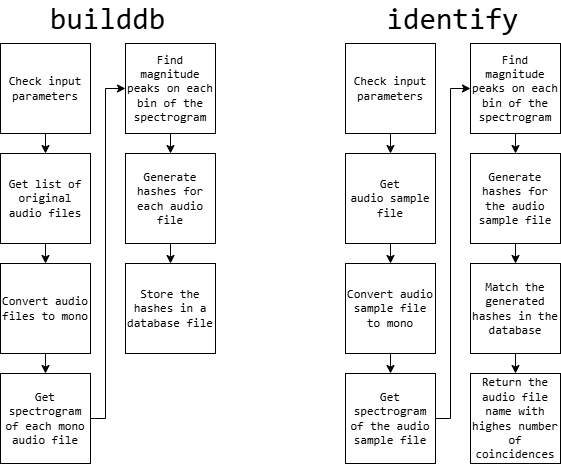
\includegraphics[width=\textwidth]{media/builddb_identify_block_diagram.png}
        \caption{Modules builddb and identify work flow}
        \label{fig:builddb_identify_block_diagram}
    \end{figure}

    The main idea of this process is to split each audio file in small samples and generate a hash for each one. This hash is based on the 
    magnitude peaks as a representative characteristic of the sample. This is done for each audio file and all the hashes are stored in a file 
    that works as a database. During the identification, the same process is carried out with the provided audio sample and then the resultant 
    hashes are collated with the database.

    \newpage

    \subsection{Module \texttt{builddb}}

    The module \texttt{builddb} is responsible for generating the audio fingerprint database. It takes as input a directory with original audio 
    tracks and produces a serialized file containing the fingerprints of all the tracks. The process is based on the Shazam fingerprinting 
    algorithm \cite{ShazamAlgorithmPaper}, and the core tasks are implemented in a state-driven manner, as shown in the flow diagram in 
    Figure~\ref{fig:builddb_identify_block_diagram}.

    \begin{enumerate}
        \item \textbf{CHECK\_INPUT\_PARAMETERS}: Validates the command-line arguments.
        \item \textbf{READ\_SONGS\_LIST}: Retrieves the original audio files and stores their names and paths.
        \item \textbf{CREATE\_FOLDERS}: Generates folders for storing mono audio and spectrograms.
        \item \textbf{CONVERT\_SONGS\_TO\_MONO}: Converts stereo audio files to mono using \texttt{NAudio}, by averaging both channels. (see Figure~\ref{fig:mono_conversion}).
        \begin{figure}[H]
            \centering
            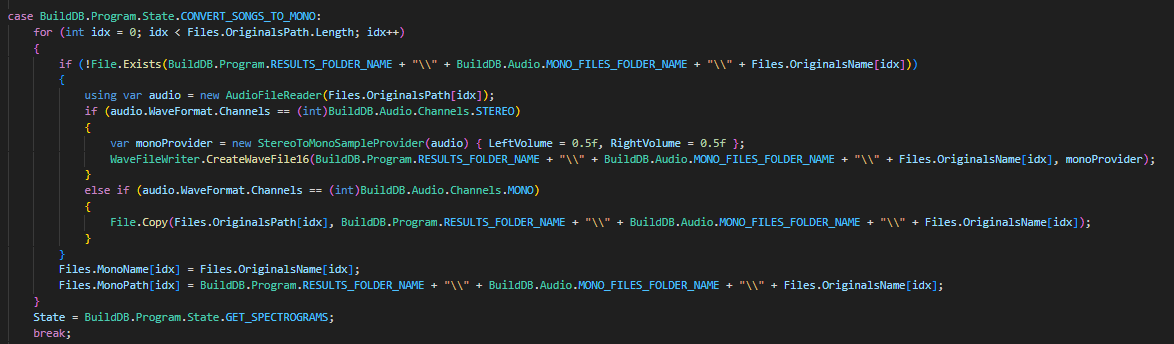
\includegraphics[width=0.9\textwidth]{media/stereo_to_mono.png}
            \caption{Stereo to mono conversion avaraging both channels using NAudio}
            \label{fig:mono_conversion}
        \end{figure}
        \item \textbf{GET\_SPECTROGRAMS}: Computes the magnitude spectrogram for each mono audio track using the Short-Time Fourier Transform (STFT) \newline from \texttt{NWaves} \cite{nwaves}. 
        For this step, each signal is segmented into overlapping frames of size $8192$ samples (defined as \texttt{SPECTROGRAM\_WINDOWS\_SIZE}) with a hop size of $4096$ samples between 
        frames (\texttt{SPECTROGRAM\_HOP\_SIZE}). A Hann window function is applied to each frame to minimize spectral leakage. Only the magnitude component of the STFT is kept, 
        discarding the phase information. The magnitude componenet is sufficient for detecting frequency peaks. The resulting time-frequency representation allows identification of l
        ocal amplitude maxima (peaks) in both the time and frequency domains, which are used in the following step. The spectrograms are serialized using the \texttt{MessagePack}.
        \begin{figure}[H]
            \centering
            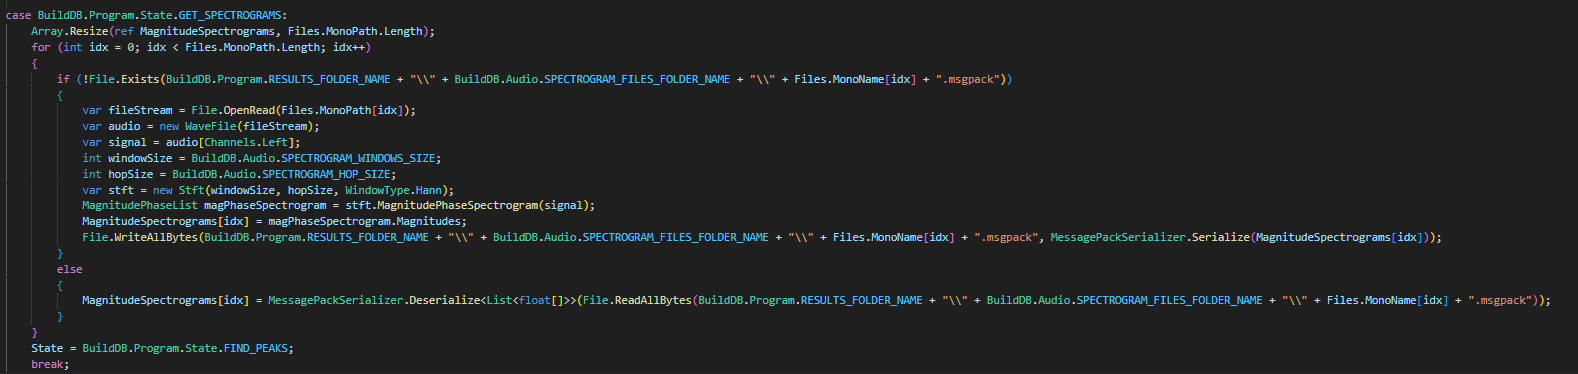
\includegraphics[width=0.9\textwidth]{media/get_spectrograms.png}
            \caption{Spectrograms obtained using NWaves}
            \label{fig:get_spectrograms}
        \end{figure}
        \item \textbf{FIND\_PEAKS}: In this step, local peaks are detected across each time frame of the magnitude spectrogram. The objective is to isolate significant frequency 
        components that are likely to be robust under noise, filtering, or distortion. A local peak is defined as a frequency bin whose amplitude is higher than its surrounding 
        neighbours within a radius of two bins (\texttt{IsLocalPeak} method) (see Figure~\ref{fig:is_local_peak}), and which exceeds a minimum amplitude threshold 
        (\texttt{MIN\_PEAK\_AMPLITUDE} = 10.0). For each frame:
        \begin{figure}[H]
            \centering
            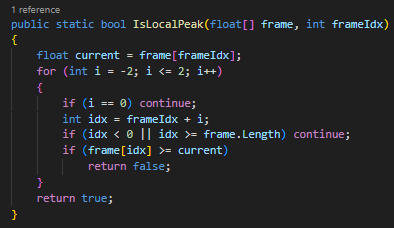
\includegraphics[width=0.5\textwidth]{media/is_local_peak.png}
            \caption{Function to detect the peaks within neighbours in a radius of two bins}
            \label{fig:is_local_peak}
        \end{figure}
        \begin{itemize}
            \item All candidate peaks are collected if they meet both criteria (local maximum and amplitude threshold).
            \item These candidates are sorted by magnitude.
            \item Only the top 10 peaks (\texttt{MAX\_PEAKS\_PER\_FRAME}) are retained per frame.
        \end{itemize}
        \item \textbf{GENERATE\_HASHES}: Fingerprints are generated by pairing each selected peak (referred to as an anchor) with other peaks within a target zone defined by frequency 
        and time distance thresholds. The pairing process follows the next rules:
        \begin{itemize}
            \item For each anchor point , other peaks are considered within a window of frames and  bins.
            \item A hash is then created that encodes the frequency of the anchor, the frequency of the target peak, and the time delta.
            \item A track ID and anchor time offset are also stored alongside the hash.
            \item For efficiency, a maximum of 10,000 hashes are generated per track \newline (\texttt{MAX\_HASHES\_PER\_TRACK}).
        \end{itemize}
        The final hash format uses bit-shifting and masking to combine the frequency and time delta into a 32-bit integer:
        \begin{equation}
            \text{hash} = (f_1 \& 0x3FF) \ll 20 \ | \ (f_2 \& 0x3FF) \ll 10 \ | \ (\Delta t \& 0x3FF)
        \end{equation}
        Where \( f_1 \) and \( f_2 \) are frequency bin indices and \( \Delta t \) is the time difference. This format is inspired by Wang's original design \cite{ShazamAlgorithmPaper}.
        \begin{figure}[H]
            \centering
            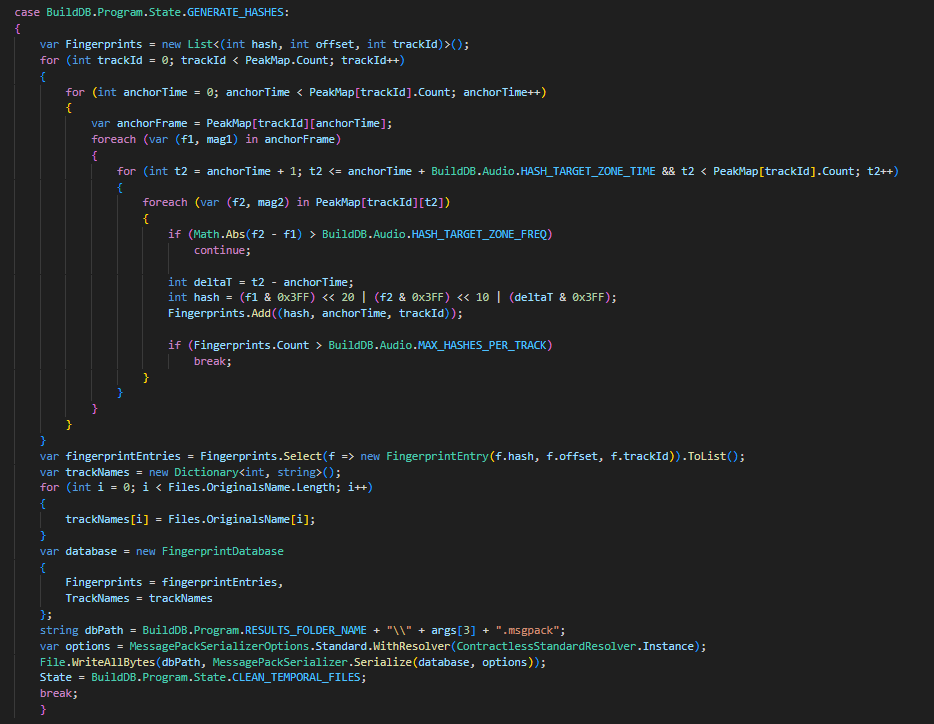
\includegraphics[width=0.5\textwidth]{media/generate_hashes.png}
            \caption{Generation of the hashes and serialization of the data}
            \label{fig:generate_hashes}
        \end{figure}
        \item \textbf{CLEAN\_TEMPORAL\_FILES}: Temporary folders containing intermediate files (e.g., mono audio, spectrograms) are deleted to reduce storage footprint.
        \item \textbf{SUCCESS}: Final state. A compact \texttt{MessagePack}-serialized fingerprint database is saved, ready for matching in the \texttt{identify} module.
    \end{enumerate}
    
    The resultant database contains a list of fingerprints and their associated data (offset and track ID), as well as a mapping from track IDs to their original filenames. This is stored in 
    an object of type \texttt{FingerprintDatabase}, which includes:
        \begin{itemize}
            \item A list of \texttt{FingerprintEntry} instances (hash, offset, trackId).
            \item A dictionary mapping track IDs to audio filenames.
        \end{itemize}

    \subsection{Module \texttt{identify}}

    The module \texttt{identify} is responsible for determining the original audio track that best matches a given sample. It takes as input a fingerprint database 
    (generated by \texttt{builddb}) and an audio sample. The module extracts fingerprints from the sample and performs matching to identify the source track.

    \begin{enumerate}
        \item \textbf{CHECK\_INPUT\_PARAMETERS}: Verifies that the arguments include a valid fingerprint database path and an input audio file.
        \item \textbf{READ\_SONG}: Loads the input file and initializes metadata. As the identification is done for a single file, arrays for paths and names contain only one element.
        \item \textbf{CREATE\_FOLDERS}: Creates temporary folders for mono audio and spectrogram if they do not already exist.
        \item \textbf{CONVERT\_SONG\_TO\_MONO}: Converts the input audio to mono using the same logic as in \texttt{builddb}.
        \item \textbf{GET\_SPECTROGRAMS}: Computes or loads the magnitude spectrogram of the sample using the same STFT parameters as in \texttt{builddb}:
        \begin{itemize}
            \item Window size: 8192 samples
            \item Hop size: 4096 samples
            \item Window function: Hann
        \end{itemize}
        The same spectral resolution is used for matching.
        \item \textbf{FIND\_PEAKS}: Local peaks in the spectrogram are extracted using the same criteria (amplitude threshold and neighborhood comparison) as the database fingerprints.
        \item \textbf{GENERATE\_HASHES}: Fingerprints are generated from the extracted peaks by pairing each anchor point with nearby peaks within the time-frequency target zone. The same 32-bit hash 
        construction is used.
        \item \textbf{LOAD\_DB}: The fingerprint database is loaded from disk and deserialized using \newline \texttt{MessagePack}.The resulting object is of type \texttt{FingerprintDatabase}, which includes:
        \begin{itemize}
            \item A list of \texttt{FingerprintEntry} instances (hash, offset, trackId).
            \item A dictionary mapping track IDs to audio filenames.
        \end{itemize}
        \begin{figure}[H]
            \centering
            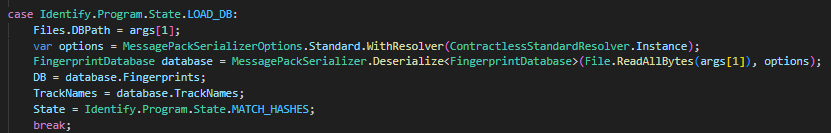
\includegraphics[width=0.5\textwidth]{media/load_db.png}
            \caption{Load of the MessagePack database}
            \label{fig:load_db}
        \end{figure}        
        \item \textbf{MATCH\_HASHES}: The list of sample hashes is compared against the loaded database. The algorithm constructs an index of the database by grouping fingerprints by hash value. Then, 
        for each hash in the sample:
        \begin{itemize}
            \item If the hash exists in the database, it retrieves a list of matching fingerprints.
            \item For each match, it computes the time offset difference \( \Delta t = t_{db} - t_{sample} \).
            \item It increments a vote for the pair \texttt{(trackId, \(\Delta t\))}.
        \end{itemize}
        After all votes are counted, the best match is determined by finding the \texttt{trackId} with the highest number of aligned matches (votes). This voting strategy is based on the technique used in the Shazam algorithm \cite{ShazamAlgorithmPaper}.
        Finally it returns to the console:
        \begin{itemize}
            \item The ID of the most probable matching track.
            \item The number of matching fingerprint alignments.
            \item The filename retrieved from \texttt{TrackNames}, if available.
        \end{itemize}
        If no strong match is found (i.e., no hash overlaps), the system reports that no match could be determined.
        \begin{figure}[H]
            \centering
            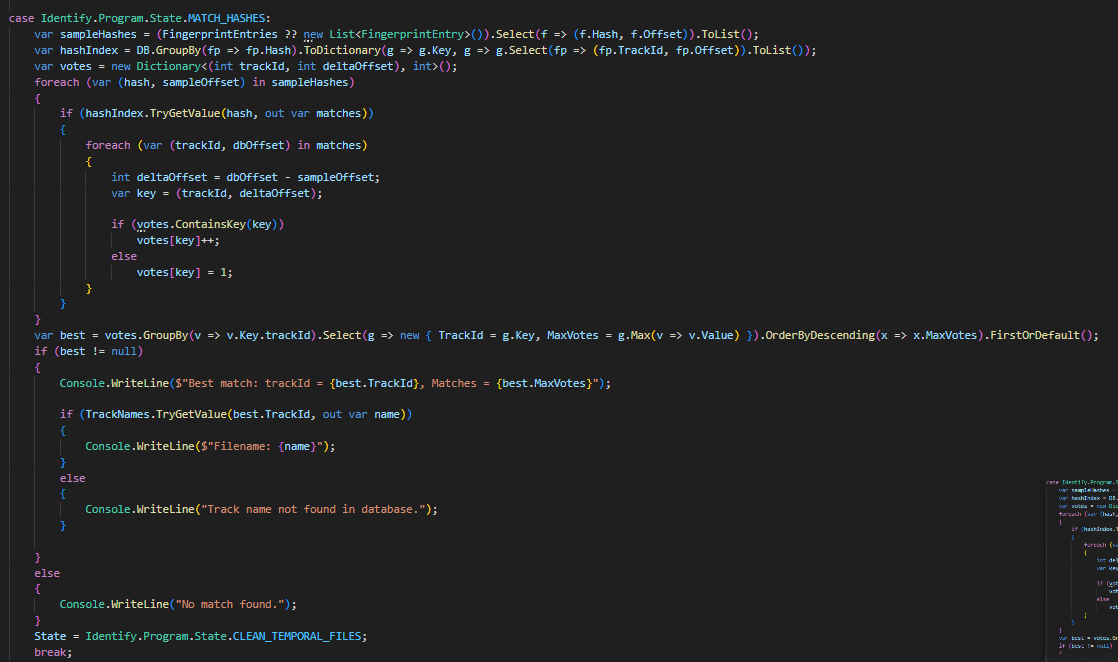
\includegraphics[width=0.5\textwidth]{media/match_hashes.png}
            \caption{Code for match and vote for the candidate TrackId}
            \label{fig:match_hashes}
        \end{figure}  
        \item \textbf{CLEAN\_TEMPORAL\_FILES}: Deletes temporary mono and spectrogram files used during processing.
        \item \textbf{SUCCESS}: The match result is printed, and the program terminates.     
    \end{enumerate}   
    The \texttt{identify} module mirrors the operations of \texttt{builddb} to compare the samples and originals fingerprints. 
    
    \subsection{Fingerprint Database Structure}

    \begin{figure}[H]
        \centering
        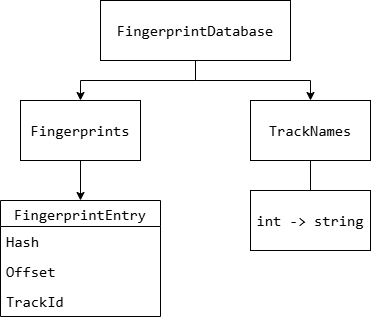
\includegraphics[width=0.5\textwidth]{media/database_structure.png}
        \caption{Structure of the \texttt{FingerprintDatabase} with Fingerprints and TrackNames}
        \label{fig:database_structure}
    \end{figure}

    The fingerprint database is a data structure serialized in the \texttt{MessagePack} format. It is created by the \texttt{builddb} module and read by the \texttt{identify} module for comparison.
    It contains the following main components:

    \begin{itemize}
        \item \textbf{Fingerprints}: A list of records where each record contains:
        \begin{itemize}
            \item \texttt{Hash}: A 32-bit integer fingerprint hash.
            \item \texttt{Offset}: The time offset (in frames) of the anchor point in the original track.
            \item \texttt{TrackId}: An integer identifying the audio track.
        \end{itemize}
        \item \textbf{TrackNames}: A dictionary mapping each \texttt{TrackId} to its corresponding audio filename.
    \end{itemize}

    Each fingerprint is stored using the \texttt{FingerprintEntry} type, defined as a serializable record. The complete database is in the \texttt{FingerprintDatabase} class.
    The use of \texttt{MessagePack} allows the creations of minimal file size and fast binary serialization/deserialization compared to textual formats like JSON. With JSON memory expections
    were thrown due to the high amount of data in the database. An example layout is shown in Figure~\ref{fig:database_structure}.

    \newpage

    \section{Testing}

    To test the application first the database must be built using the program \texttt{builddb.exe}. For this the following command has to be executed:

    \vspace{1em} \texttt{builddb.exe -i <path\_to\_folder\_with\_audio\_files> -o <name\_of\_the\_database\_generated>}

    \vspace{1em} The resultant database file with extension \texttt{.msgpack} is stored in the folder \texttt{results} that will be created in the same directory as the \texttt{builddb.exe} during the execution. 
    In the testing computer (AMD Ryzen 5 2600 @ 3.8Ghz - 16 GB RAM DD3 @ 2166 Mhz) takes around 65 and 68 seconds to complete the process.

    \begin{figure}[H]
        \centering
        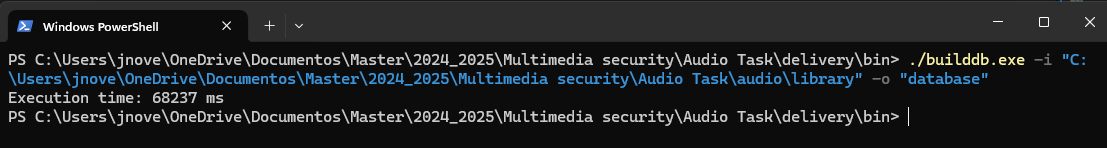
\includegraphics[width=\textwidth]{media/buildb_execution.png}
        \caption{Successful execution of the builddb program.}
        \label{fig:buildb_execution}
    \end{figure}

    Once the database is created the identification process can be carried out with the program \texttt{identify.exe}. To use it the next command must be executed:

    \vspace{1em} \texttt{identify.exe -d <path\_to\_the\_database\_file> -i <path\_to\_sample\_audio\_files>}

    \vspace{1em} The Successful rate with the tests done is 100\%. The program has not been teste with all the samples available but all the test done have been successful. The time
    taken for the identification is always around 60-70 seconds. In the following image some random test are done with clean, filtered, noisy and noisy filtered samples.

    \begin{figure}[H]
        \centering
        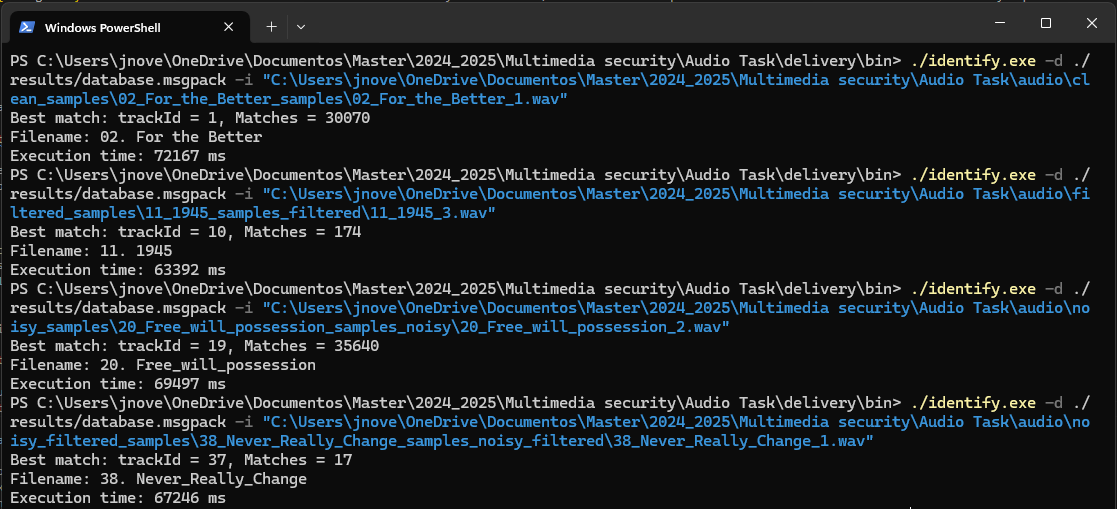
\includegraphics[width=\textwidth]{media/identify_execution.png}
        \caption{Successful execution of the identify program.}
        \label{fig:identify_execution}
    \end{figure}

    \newpage

    \begin{thebibliography}{11}

    \bibitem{ShazamAlgorithmPaper}
    A. L.-C. Wang, \textit{An Industrial-Strength Audio Search Algorithm}.  
    Shazam Entertainment, Ltd.  
    Available at \url{https://www.ee.columbia.edu/~dpwe/papers/Wang03-shazam.pdf}.

    \bibitem{PythonVsCSharp}
    TCM Security, \textit{Python vs C\# \newline Which One is Better in 2023?}.  
    Available at \url{https://tcm-sec.com/python-vs-c-sharp/#:~:text=Performance%20and%20Speed,only%202%20seconds%20to%20run}.

    \bibitem{nwaves}
    NWaves DSP Library. Available at \url{https://github.com/ar1st0crat/NWaves}

    \bibitem{aubio}
    P. Brossier, \textit{Automatic annotation of musical audio for interactive systems}. 
    PhD Thesis, Queen Mary University of London, 2006.

    \bibitem{zhu2008}
    Y. Zhu and D. P. W. Ellis, \textit{Estimating the similarity of short music excerpts using feature rank histograms}. 
    In Proceedings of the 2008 IEEE International Conference on Acoustics, Speech and Signal Processing (ICASSP), pp. 1337–1340.

\end{thebibliography}

\end{document}
